%============================================================
%  Capitolo 4 – Loss Functions
%============================================================
\chapter{Loss Functions}
\label{ch:loss-functions}

La \textbf{funzione di perdita} (loss function, o cost function) misura la discrepanza
tra la previsione della rete e il target desiderato. La scelta della loss è tanto
importante quanto quella dell'architettura: determina \textit{cosa} la rete impara
ad ottimizzare, e influenza il comportamento del gradiente durante il training.

In PyTorch tutte le loss sono implementate nel modulo \texttt{torch.nn} e seguono
una convenzione comune: accettano un input \texttt{x} (la predizione) e un target
\texttt{y}, e supportano l'argomento \texttt{reduction} (\texttt{'none'},
\texttt{'mean'}, \texttt{'sum'}) per controllare come le loss elementari vengono
aggregate sul batch \citep{bishop2024}.

%------------------------------------------------------------
\section{Loss per Regressione}
\label{sec:regression-losses}

\subsection{MSE Loss -- \texttt{nn.MSELoss()}}
\label{subsec:mse}

La \textbf{Mean Squared Error} (errore quadratico medio, norma L2 al quadrato)
è la loss di regressione più comune:

\begin{equation}
  l(x, y) = L = \{l_1, \ldots, l_N\}^\top, \qquad
  l_n = (x_n - y_n)^2,
\end{equation}

dove $N$ è la dimensione del batch. Con \texttt{reduction='none'} la loss viene
restituita come vettore; altrimenti:

\begin{equation}
  l(x, y) =
  \begin{cases}
    \operatorname{mean}(L), & \text{se reduction} = \texttt{'mean'} \\
    \operatorname{sum}(L),  & \text{se reduction} = \texttt{'sum'}
  \end{cases}
\end{equation}

La somma opera su tutti gli elementi e, con \texttt{'mean'}, divide per $n$.
Per evitare la divisione si usa \texttt{reduction='sum'}.

\paragraph{Pro e contro.}
MSE è differenziabile ovunque e penalizza fortemente gli errori grandi (il quadrato
amplifica gli outlier). In task di regressione con output continui è la scelta
predefinita, ma soffre di elevata sensibilità al rumore.

\subsection{L1 Loss -- \texttt{nn.L1Loss()}}
\label{subsec:l1}

La \textbf{Mean Absolute Error} (MAE) misura l'errore assoluto medio:

\begin{equation}
  l(x, y) = L = \{l_1, \ldots, l_N\}^\top, \qquad
  l_n = |x_n - y_n|.
\end{equation}

Supporta le stesse opzioni di riduzione di \texttt{nn.MSELoss()}.

\paragraph{Vantaggio rispetto a L2.}
L1 è più robusta agli outlier: gli errori non vengono elevati al quadrato, quindi
i punti rumorosi influenzano meno la loss totale. Il valore $y$ che minimizza la
distanza L1 è la \textbf{mediana} (anziché la media per L2), il che produce
predizioni meno sfocate in task come la super-risoluzione d'immagine.

\begin{quote}
\textit{L1 ha gradienti costanti: anche quando la loss si avvicina a zero,
il gradiente non si annulla, producendo immagini predette più nitide.}
\end{quote}

\paragraph{Limite.}
L1 \textbf{non è differenziabile in} $x=0$ (dove la funzione valore assoluto ha
un ``angolo''). Questo richiede attenzione nella gestione del gradiente
(cfr.\ \texttt{nn.Softshrink}). Per questo motivo è stata introdotta la
SmoothL1Loss.

\subsection{Smooth L1 Loss (Huber Loss) -- \texttt{nn.SmoothL1Loss()}}
\label{subsec:smooth-l1}

Combina L2 per errori piccoli e L1 per errori grandi, eliminando il problema
della non-differenziabilità in zero:

\begin{equation}
  \operatorname{loss}(x, y) = \frac{1}{n}\sum_i z_i, \qquad
  z_i =
  \begin{cases}
    0.5\,(x_i - y_i)^2,   & \text{se } |x_i - y_i| < 1 \\
    |x_i - y_i| - 0.5,    & \text{altrimenti}
  \end{cases}
\end{equation}

Nota anche come \textbf{Huber Loss} o \textbf{Elastic Network} quando usata come
funzione obiettivo. È stata resa popolare da Ross Girshick in Fast R-CNN.

\paragraph{Pro e contro.}
Meno sensibile agli outlier rispetto a MSE e smooth nel punto zero.
Usata frequentemente in \textbf{computer vision} (object detection) per
proteggere contro outlier nelle coordinate dei bounding box.
Il limite è la presenza del fattore di scala $0.5$ fisso nella regione quadratica.

\subsection{L1 vs.\ L2 in Computer Vision}
\label{subsec:l1-l2-cv}

In task di predizione d'immagine dove esistono molte possibili output $y$:

\begin{itemize}
  \item \textbf{MSE (L2)}: la previsione converge alla \textit{media} di tutte
        le possibili $y$. In visione artificiale questo produce immagini
        \textbf{sfocate} (blur), perché la media di immagini nitide con
        strutture leggermente diverse è un'immagine priva di dettagli.
  \item \textbf{L1}: la previsione converge alla \textit{mediana}, che non
        produce blur ma è difficile da definire in spazi multidimensionali.
\end{itemize}

\begin{figure}[H]
  \centering
  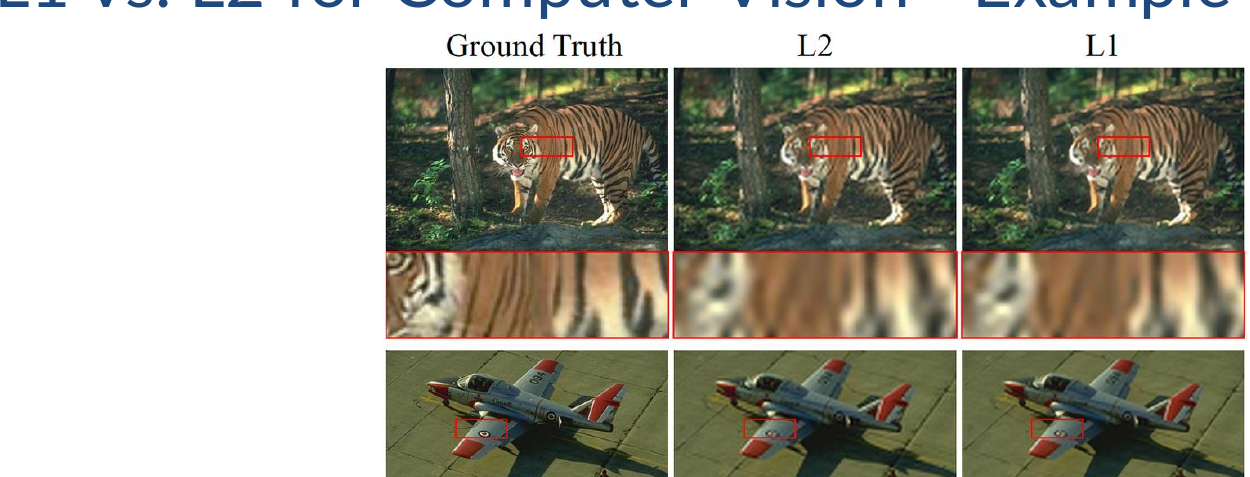
\includegraphics[width=0.82\linewidth]{figures/cf04_l1l2_cv_example.png}
  \caption{Confronto visivo tra Ground Truth, predizione con L2 (sfocata) e
           predizione con L1 (più nitida) su due esempi: una tigre e un aereo.
           Il dettaglio ingrandito mostra come L2 produca un'area blurred nel
           crop della tigre, mentre L1 preserva meglio le strutture.
           [Fonte: towardsdatascience.com/perceptual-losses-for-image-restoration]}
  \label{fig:l1l2_cv}
\end{figure}

%------------------------------------------------------------
\section{Loss per Classificazione}
\label{sec:classification-losses}

\subsection{NLL Loss -- \texttt{nn.NLLLoss()}}
\label{subsec:nll}

La \textbf{Negative Log Likelihood Loss} è usata per problemi di classificazione
con $C$ classi. Matematicamente, l'input dovrebbe essere una log-likelihood
(come l'output di \texttt{nn.LogSoftmax}), ma PyTorch non lo impone.

Loss non ridotta:
\begin{equation}
  l(x, y) = L = \{l_1, \ldots, l_N\}^\top, \qquad
  l_n = -w_{y_n}\, x_{n,\, y_n}, \qquad
  w_c = \operatorname{weight}[c] \cdot \mathbf{1}\{c \neq \texttt{ignore\_index}\}.
\end{equation}

Con riduzione:
\begin{equation}
  l(x,y) =
  \begin{cases}
    \displaystyle\sum_{n=1}^{N} \frac{1}{\sum_{n=1}^{N} w_{y_n}} l_n,
      & \text{se reduction} = \texttt{'mean'} \\[6pt]
    \displaystyle\sum_{n=1}^{N} l_n,
      & \text{se reduction} = \texttt{'sum'}
  \end{cases}
\end{equation}

L'argomento opzionale \textbf{weight} accetta un tensore 1D che assegna un peso
a ciascuna classe, utile per gestire dataset sbilanciati.

\subsection{Gestione dei Dataset Sbilanciati}
\label{subsec:imbalanced}

Quando la frequenza delle classi differisce notevolmente (es.\ influenza comune vs
cancro al polmone), si possono adottare due strategie:

\paragraph{Strategia 1 -- Pesi nella loss.}
Aumentare il peso \texttt{weight[c]} per le classi minoritarie in \texttt{NLLLoss}
o \texttt{CrossEntropyLoss}.

\paragraph{Strategia 2 -- Equalizzazione della frequenza (preferita).}
Invece di assegnare pesi, è meglio \textbf{equalizzare la frequenza nel training}
per sfruttare meglio i gradienti stocastici:
\begin{enumerate}
  \item Raccogliere i campioni di ogni classe in buffer separati.
  \item Generare ogni minibatch prendendo lo stesso numero di campioni da ciascun
        buffer.
  \item Quando il buffer della classe minoritaria si esaurisce, ricominciare
        dall'inizio (buffer circolare) finché tutti i campioni della classe
        maggioritaria sono stati usati.
\end{enumerate}

\textbf{Attenzione}: non ridurre artificialmente la classe maggioritaria scartando
campioni --- non sprecare dati. Se si equalizza la frequenza, il modello non
conosce più la frequenza reale delle classi. Per correggere questo, si eseguono
pochi epoch finali con la distribuzione reale delle classi, affinché il sistema
adatti i bias dell'output layer.

\subsection{Cross-Entropy Loss -- \texttt{nn.CrossEntropyLoss()}}
\label{subsec:cross-entropy}

Combina \texttt{nn.LogSoftmax} e \texttt{nn.NLLLoss} in un'unica classe,
massimizzando lo score della classe corretta:

\begin{equation}
  \operatorname{loss}(x, c) =
  -\log\!\left(\frac{\exp(x[c])}{\sum_j \exp(x[j])}\right)
  = -x[c] + \log\!\left(\sum_j \exp(x[j])\right).
\end{equation}

Con peso per classe $w[c]$:
\begin{equation}
  \operatorname{loss}(x, c) = w[c]\!\left(-x[c] + \log\!\left(\sum_j \exp(x[j])\right)\right).
\end{equation}

\paragraph{Perché unire LogSoftmax e NLLLoss?}
Quando il valore dopo Softmax è vicino a $0$ o $1$, il suo logaritmo tende a
$-\infty$ e la derivata del $\log$ vicino a $0$ tende a $+\infty$, causando
instabilità numerica durante la retropropagazione. Unendo le due operazioni,
i gradienti vengono saturati a valori ragionevoli tramite il \textbf{log-sum-exp trick}.

\paragraph{Interpretazione probabilistica: KL Divergence.}
La Cross-Entropy ha una lettura information-theoretic: misura la
\textbf{divergenza di Kullback-Leibler} tra la distribuzione predetta $q$ e
quella target $p$:

\begin{align}
  H(p, q) &= H(p) + \mathcal{D}_{KL}(p \,\|\, q) \\
  H(p, q) &= -\sum_i p(x_i)\log q(x_i) \qquad \text{(cross-entropy)} \\
  H(p)    &= -\sum_i p(x_i)\log p(x_i) \qquad \text{(entropia)} \\
  \mathcal{D}_{KL}(p\|q) &= \sum_i p(x_i)\log\frac{p(x_i)}{q(x_i)} \quad \text{(KL divergence)}
\end{align}

Nel caso classificazione, $p$ è il vettore one-hot (0 sulle classi errate, 1 sulla
corretta) e $q$ è il vettore Softmax delle predizioni. Minimizzare la Cross-Entropy
equivale a minimizzare la KL Divergence tra predizioni e target.

\subsection{Binary Cross Entropy -- \texttt{nn.BCELoss()}}
\label{subsec:bce}

Caso speciale della Cross-Entropy per \textbf{due classi}:

\begin{equation}
  l(x, y) = L = \{l_1, \ldots, l_N\}^\top, \qquad
  l_n = -w_n\bigl[y_n \log x_n + (1-y_n)\log(1-x_n)\bigr].
\end{equation}

Usata tipicamente per misurare l'errore di ricostruzione in un auto-encoder.
\textbf{Attenzione}: la formula assume che $x$ e $y$ siano probabilità, quindi
strettamente in $(0, 1)$.

\subsection{BCE with Logits -- \texttt{nn.BCEWithLogitsLoss()}}
\label{subsec:bce-logits}

Versione numericamente più stabile di BCELoss: accetta score grezzi (logit) non
normalizzati e applica internamente la Sigmoid prima del log:

\begin{equation}
  l_n = -w_n\bigl[y_n \log\sigma(x_n) + (1-y_n)\log(1-\sigma(x_n))\bigr].
\end{equation}

Non assume che $x \in (0,1)$ e combina Sigmoid + BCE in un'unica operazione
numericamente stabile. \textbf{È preferita a \texttt{nn.BCELoss}} nelle reti con
output layer lineare.

\subsection{NLL Loss Adattiva -- \texttt{nn.AdaptiveLogSoftmaxWithLoss()}}
\label{subsec:adaptive}

Approssimazione efficiente di Softmax per un numero molto elevato di classi
(nell'ordine dei milioni). Implementa il metodo descritto in
\textit{Efficient softmax approximation for GPUs} (Grave et al., 2017), che
raggruppa le classi per frequenza e usa head di dimensioni diverse per classi
rare vs frequenti.

\subsection{KL Divergence Loss -- \texttt{nn.KLDivLoss()}}
\label{subsec:kldiv}

\begin{equation}
  l(x, y) = L = \{l_1, \ldots, l_N\}^\top, \qquad
  l_n = y_n(\log y_n - \log x_n).
\end{equation}

Utile quando il target è una distribuzione one-hot. Assume che $x$ e $y$ siano
probabilità. \textbf{Svantaggio}: non è integrata con una Softmax o LogSoftmax,
quindi può soffrire di instabilità numerica. Per questo motivo si preferisce
\texttt{nn.CrossEntropyLoss} nella maggior parte dei casi.

%------------------------------------------------------------
\section{Loss Basate su Margine}
\label{sec:margin-losses}

Le \textbf{margin losses} sono una categoria importante di loss functions: invece
di misurare la distanza assoluta tra predizione e target, richiedono che la
predizione corretta superi quella errata di almeno un certo margine.

\subsection{Hinge Embedding Loss -- \texttt{nn.HingeEmbeddingLoss()}}
\label{subsec:hinge-embedding}

Usata in apprendimento semi-supervisionato per misurare la similarità/dissimilarità
tra coppie di input:

\begin{equation}
  l_n =
  \begin{cases}
    x_n,                        & y_n = 1  \\
    \max\{0,\, \delta - x_n\},  & y_n = -1
  \end{cases}
\end{equation}

La variabile $y$ indica se la coppia $(x)$ è simile ($+1$) o dissimile ($-1$).
Con la hinge loss, lo score è positivo se $y=1$ e viene penalizzato se $y=-1$
ma non supera il margine $\delta$.
Di solito si usa con la distanza L1 a coppie come $x$.

\subsection{Margin Ranking Loss -- \texttt{nn.MarginRankingLoss()}}
\label{subsec:margin-ranking}

\begin{equation}
  L(x, y) = \max\bigl(-y \cdot (x_1 - x_2) + \operatorname{margin},\; 0\bigr).
\end{equation}

Richiede che un input sia maggiore dell'altro di almeno \texttt{margin}:
\begin{itemize}
  \item $x_1, x_2$: score assegnati dalla rete a due item (positivo e negativo).
  \item $y = +1$: si vuole $x_1 > x_2$ (item positivo deve avere score maggiore).
  \item $y = -1$: si vuole $x_2 > x_1$ (flip del confronto).
  \item \texttt{margin}: soglia minima della differenza desiderata tra gli score.
\end{itemize}

Se $y \cdot (x_1 - x_2) > \operatorname{margin}$, il costo è $0$; altrimenti
cresce linearmente. In classificazione, $x_1$ è lo score della risposta corretta
e $x_2$ è lo score più alto tra le risposte errate nel minibatch.
Nei modelli energy-based (EBM), questa loss abbassa l'energia della risposta
corretta $x_1$ e alza quella della risposta errata $x_2$.

\subsection{Triplet Margin Loss -- \texttt{nn.TripletMarginLoss()}}
\label{subsec:triplet}

\begin{equation}
  L(a, p, n) = \max\bigl\{d(a_i, p_i) - d(a_i, n_i) + \operatorname{margin},\; 0\bigr\},
\end{equation}

dove $a$ è l'anchor, $p$ è il campione positivo (stessa classe), $n$ è quello
negativo (classe diversa) e $d(\cdot, \cdot)$ è una metrica di distanza.

Usata per misurare similarità relativa tra campioni:
\begin{itemize}
  \item Due immagini della stessa categoria passate a una CNN devono produrre
        vettori \textbf{vicini}.
  \item Due immagini di categorie diverse devono produrre vettori
        \textbf{lontani}.
\end{itemize}

La loss spinge la distanza della coppia positiva verso $0$ e quella della coppia
negativa oltre il margine. Ciò che conta è che la distanza della coppia buona sia
\textit{minore} di quella della coppia cattiva, non i valori assoluti.

\subsection{Soft Margin Loss -- \texttt{nn.SoftMarginLoss()}}
\label{subsec:soft-margin}

\begin{equation}
  L(x, y) = \sum_i \frac{\log\bigl(1 + \exp(-y[i] \cdot x[i])\bigr)}{n.\mathrm{nelement}()}.
\end{equation}

Versione \textbf{soft} (continua) della margin loss: ottimizza una perdita
logistica per classificazione a due classi con target $y \in \{-1, +1\}$.
Vuole che $\exp(-y[i] \cdot x[i])$ per la risposta corretta sia più piccolo che
per le altre: avvicina i valori positivi di $y[i] \cdot x[i]$ e allontana quelli
negativi, ma con un effetto esponenzialmente decrescente (a differenza di un hard
margin).

\subsection{Multi-Class Hinge Loss -- \texttt{nn.MultiLabelMarginLoss()}}
\label{subsec:multilabel-margin}

\begin{equation}
  L(x, y) = \sum_{ij} \frac{\max\bigl(0,\; 1 - (x[y[j]] - x[i])\bigr)}{x.\mathrm{size}(0)}.
\end{equation}

Estende la hinge loss al caso multiclasse, permettendo a diversi input di avere
quantità variabili di target. Somma la hinge loss su tutte le categorie target.
Nei modelli EBM, abbassa l'energia delle categorie desiderate e alza quella delle
non-desiderate.

%------------------------------------------------------------
\section{Loss per Embedding: Cosine Embedding Loss}
\label{sec:cosine-embedding}

\subsection{Formulazione}
\label{subsec:cosine-formula}

\texttt{nn.CosineEmbeddingLoss()} misura se due input sono simili o dissimili
usando la \textbf{distanza coseno}:

\begin{equation}
  l_n =
  \begin{cases}
    1 - \cos(x_1, x_2),                      & y = 1  \\
    \max\{0,\; \cos(x_1, x_2) - \operatorname{margin}\}, & y = -1
  \end{cases}
\end{equation}

Tipicamente usata per apprendere embedding non lineari o in apprendimento
semi-supervisionato.

\begin{figure}[H]
  \centering
  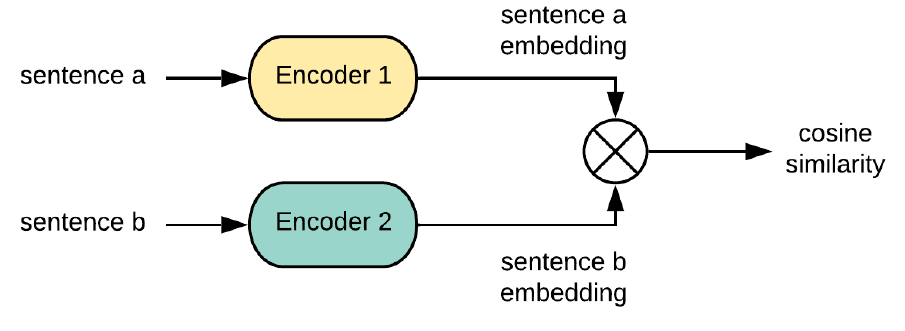
\includegraphics[width=0.68\linewidth]{figures/cf04_cosine_encoder_diagram.png}
  \caption{Schema della CosineEmbeddingLoss: due input (\textit{sentence a} e
           \textit{sentence b}) vengono proiettati attraverso due encoder e i
           rispettivi embedding vengono confrontati tramite cosine similarity.
           Il simbolo $\otimes$ indica il prodotto scalare normalizzato.}
  \label{fig:cosine_encoder}
\end{figure}

\subsection{Interpretazione Geometrica}
\label{subsec:cosine-geometry}

$1 - \cos(\theta)$ tra due vettori è equivalente alla \textbf{distanza euclidea
normalizzata}: dopo aver portato i vettori sulla sfera unitaria, la loro distanza
dipende solo dall'angolo $\theta$ tra loro, non dalla loro norma.

\begin{figure}[H]
  \centering
  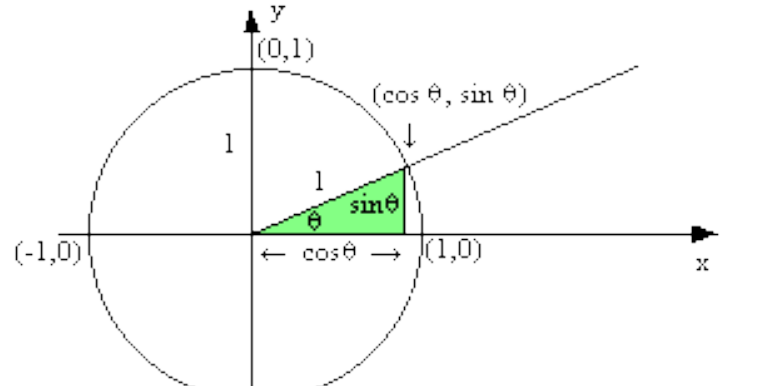
\includegraphics[width=0.52\linewidth]{figures/cf04_cosine_unit_circle.png}
  \caption{Cerchio unitario: il punto $(\cos\theta, \sin\theta)$ giace sulla
           sfera unitaria. La distanza coseno $1 - \cos\theta$ misura quanto
           due vettori normalizzati differiscono in direzione, indipendentemente
           dalla loro magnitudine.}
  \label{fig:cosine_circle}
\end{figure}

\paragraph{Perché normalizzare?}
Se si vuole massimizzare la distanza tra vettori dissimili, la rete potrebbe
semplicemente allungare i vettori anziché ruotarli nella direzione corretta.
La normalizzazione forza la rete a \textbf{ruotare} i vettori, non a scalarne
la norma. In uno spazio ad alta dimensione, la maggior parte dell'``area'' della
sfera si trova vicino all'equatore: dopo la normalizzazione, campioni semanticamente
simili devono stare vicini sulla sfera, quelli dissimili devono essere
\textbf{ortogonali}.

\paragraph{Comportamento per le due casistiche:}
\begin{itemize}
  \item \textbf{Coppie positive} ($y=1$): la loss cerca di allineare i vettori
        il più possibile ($\cos\theta \to 1$).
  \item \textbf{Coppie negative} ($y=-1$): la loss spinge il coseno sotto un
        margine positivo piccolo, rendendo i vettori ortogonali o opposti.
\end{itemize}

%------------------------------------------------------------
\section{Guida Pratica alla Scelta della Loss}
\label{sec:loss-guide}

\begin{table}[H]
  \centering
  \caption{Guida alla scelta della funzione di perdita.}
  \label{tab:loss_guide}
  \small
  \begin{tabularx}{\linewidth}{l l X}
    \toprule
    \textbf{Task} & \textbf{Loss consigliata} & \textbf{Note} \\
    \midrule
    Regressione standard        & \texttt{MSELoss}             & Sensibile agli outlier \\
    Regressione robusta         & \texttt{SmoothL1Loss}        & Huber, usata in CV \\
    Regressione con immagini    & \texttt{L1Loss}              & Predizioni più nitide \\
    Classificazione multiclasse & \texttt{CrossEntropyLoss}    & Input = logit grezzi \\
    Classificazione binaria     & \texttt{BCEWithLogitsLoss}   & Numericamente stabile \\
    Classi sbilanciate          & \texttt{NLLLoss} + weight    & O equalizzare frequenza \\
    Classi $\gg 10^4$           & \texttt{AdaptiveLogSoftmax}  & Approssimazione efficiente \\
    Ranking / retrieval         & \texttt{MarginRankingLoss}   & Coppia positivo/negativo \\
    Metric learning             & \texttt{TripletMarginLoss}   & Tripla anchor/pos/neg \\
    Embedding similarity        & \texttt{CosineEmbeddingLoss} & Direzione vettoriale \\
    \bottomrule
  \end{tabularx}
\end{table}

\paragraph{Regole operative.}
\begin{enumerate}
  \item Usare sempre \texttt{nn.CrossEntropyLoss} (non \texttt{Softmax} +
        \texttt{NLLLoss} separatamente) per stabilità numerica del gradiente.
  \item Per classificazione binaria preferire \texttt{BCEWithLogitsLoss}
        a \texttt{BCELoss}: non richiedere che l'output sia già in $(0,1)$.
  \item In computer vision generativa (super-risoluzione, inpainting) preferire
        L1 a L2 per evitare immagini sfocate.
  \item Per dataset sbilanciati, privilegiare l'equalizzazione della frequenza
        sui buffer rispetto ai pesi nella loss, e fare fine-tuning finale con la
        distribuzione reale.
  \item Nelle loss basate su margine, scegliere il valore del margine tramite
        validation set: un margine troppo piccolo produce scarsa separazione, uno
        troppo grande può impedire la convergenza.
\end{enumerate}

%------------------------------------------------------------
\section{Riepilogo}
\label{sec:summary-ch4}

\begin{center}
\small
\begin{tabular}{lll}
  \toprule
  \textbf{Categoria} & \textbf{Loss} & \textbf{Proprietà chiave} \\
  \midrule
  Regressione   & MSE               & Media, sensibile outlier \\
                & L1                & Mediana, robusta, non diff.\ in 0 \\
                & SmoothL1 (Huber)  & L2 vicino a 0, L1 lontano \\
  \midrule
  Classificazione & CrossEntropyLoss & LogSoftmax + NLL fusi \\
                  & BCEWithLogitsLoss & Sigmoid + BCE fusi \\
                  & NLLLoss           & Con pesi per classi sbilanciate \\
                  & KLDivLoss         & Distanza tra distribuzioni \\
  \midrule
  Margine       & HingeEmbedding    & Similarità/dissimilarità \\
                & MarginRanking     & Ordinamento relativo \\
                & TripletMargin     & Anchor/Positivo/Negativo \\
                & CosineEmbedding   & Similarità angolare normalizzata \\
  \bottomrule
\end{tabular}
\end{center}

La scelta della loss non è separabile dall'architettura: \texttt{CrossEntropyLoss}
richiede logit grezzi in input (non una Softmax esplicita), \texttt{BCEWithLogitsLoss}
richiede logit (non probabilità), e le loss basate su margine operano su coppie o
triple che devono essere costruite correttamente nel DataLoader.
Come sottolinea \citet{bishop2024}, la loss function codifica l'assunzione
probabilistica sul rumore del dato: MSE corrisponde a un modello gaussiano,
L1 a un modello laplaciano, e la Cross-Entropy al massimo della
verosimiglianza per distribuzioni categoriali.
